\documentclass{article}
\usepackage[a4paper, total={5.4in, 9in}]{geometry}
\usepackage{graphicx}
\usepackage{float}
\usepackage{subcaption}
\usepackage{amsmath}
\usepackage{amsfonts}
\setlength{\parindent}{0pt}

\newcommand{\Tr}[1]{\text{Tr}\left\{ #1 \right\}}
\renewcommand{\Re}[1]{\mathfrak{Re}\left[ #1 \right]}
\renewcommand{\Im}[1]{\mathfrak{Im}\left[ #1 \right]}

\begin{document}

\section{Simulation result}

\begin{figure}[H]
    \centering
    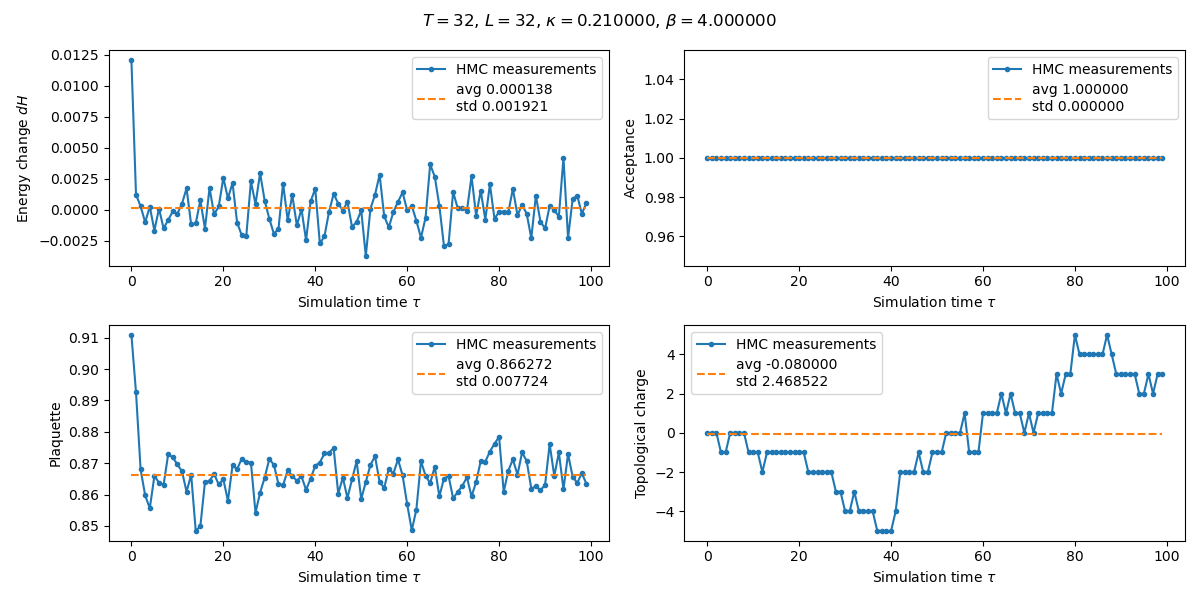
\includegraphics[width=\textwidth]{../plots/general.png}
\end{figure}

\section{Computation of two-point correlators}

We are interested to compute functions of the form $\langle j_X(r_1) j_Y(r_2) \rangle$, 
where $r_1$ and $r_2$ are positions and $X, Y$ subscripts denote the current of interest.

\begin{itemize}
    \item Vector current $j_V^{\mu, ab}(t, x) = \bar\psi_a(t, x) \gamma^\mu \psi_b(t, x)$
    \item Axial current $j_A^{\mu, ab}(t, x) = \bar\psi_a(t, x) \gamma^\mu \gamma^5 \psi_b(t, x)$
    \item Pseudoscalar current $j_P^{ab}(t, x) = \bar\psi_a(t, x) \gamma^5 \psi_b(t, x)$
\end{itemize}

Now for the computation:

\begin{itemize}
    \item We choose a reference point $r_2=0$ on the lattice (e.g. middle)
    \item We can use Wick's theorem (we discard any global sign for now) to express these two-point functions as traces in spinor space.
    \item We use the CG algorithm to solve for the propagator $S(r_1, 0)$ (inverse Dirac operator). 
\end{itemize}

We assume that the propagator is diagonal in flavour space and express the spinor components as 
\begin{equation}
    S(t, x; 0, 0) = \begin{pmatrix} S_{00} & S_{01} \\ S_{10} & S_{11} \end{pmatrix}    
\end{equation}
We also use $\gamma^5$ hermiticity (ref Gattriger \& Lang), i.e. for arbitrary $r_1, r_2$ 
\begin{equation}
    S(r_2, r_1) = \gamma^5 S(r_1, r_2)^\dagger \gamma^5
\end{equation}

Our representation of Euclidean gamma matrices:

\begin{equation}
    \gamma^0 = \begin{pmatrix} 0 & 1 \\ 1 & 0 \end{pmatrix} \hspace{10mm}
    \gamma^1 = \begin{pmatrix} 0 & -i \\ i & 0 \end{pmatrix} \hspace{10mm}
    \gamma^5 = \begin{pmatrix} 1 & 0 \\ 0 & -1 \end{pmatrix}
\end{equation}

\subsection{P-P correlator}

\begin{align*}
    \langle j_P^{12} (r) j_P^{21}(0) \rangle &= \langle \bar\psi_1(r) \gamma^5 \psi_2(r) \bar\psi_2(0) \gamma^5 \psi_1(0) \rangle \simeq \Tr{S(r, 0) \gamma^5 S(0, r) \gamma^5} \\
    &= \Tr{S(r, 0) \gamma^5 \gamma^5 S(r, 0)^\dagger \gamma^5 \gamma^5} \\
    &= \Tr{S(r, 0) S(r, 0)^\dagger} \\
    &= \Tr{ \begin{pmatrix} S_{00} & S_{01} \\ S_{10} & S_{11} \end{pmatrix} \begin{pmatrix} S_{00}^* & S_{10}^* \\ S_{01}^* & S_{11}^* \end{pmatrix} } \\
    &= \Tr{\begin{pmatrix} S_{00} S_{00}^* + S_{01} S_{01}^* &  \\ & S_{10} S_{10}^* + S_{11} S_{11}^* \end{pmatrix}} \\
    &= |S_{00}|^2 + |S_{01}|^2 + |S_{10}|^2 + |S_{11}|^2
\end{align*}

\begin{figure}[H]
    \centering
    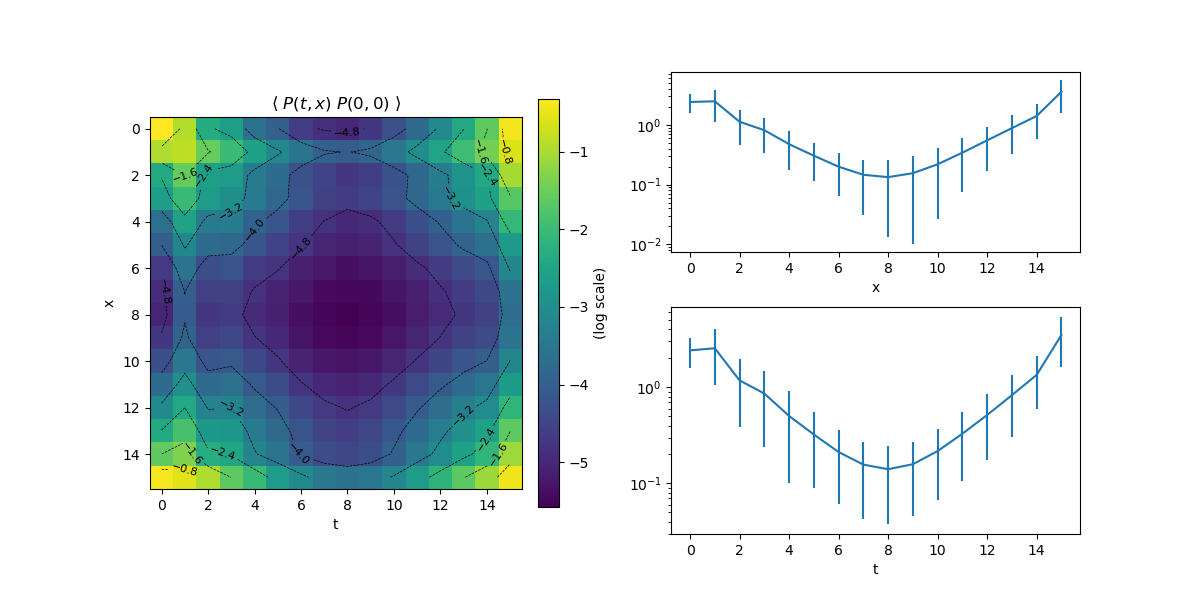
\includegraphics[width=\textwidth]{../plots/PP.png}
    \caption{}
    \label{}
\end{figure}

\subsection{A-P correlators}

\begin{align*}
    \langle j_A^{\mu, 12} (r) j_P^{21}(0) \rangle &= \langle \bar\psi_1(r) \gamma^\mu \gamma^5 \psi_2(r) \bar\psi_2(0) \gamma^5 \psi_1(0) \rangle 
    \simeq \Tr{S(r, 0) \gamma^\mu \gamma^5 S(0, r) \gamma^5} \\
    &= \Tr{S(r, 0) \gamma^\mu \gamma^5 \gamma^5 S(r, 0)^\dagger \gamma^5 \gamma^5} \\
    &= \Tr{S(r, 0) \gamma^\mu S(r, 0)^\dagger}
\end{align*}

For $\mu = 0$ we have
\begin{align*}
    \langle j_A^{0, 12} (r) j_P^{21}(0) \rangle 
    &= \Tr{ \begin{pmatrix} S_{00} & S_{01} \\ S_{10} & S_{11} \end{pmatrix} \begin{pmatrix} 0 & 1 \\ 1 & 0 \end{pmatrix} \begin{pmatrix} S_{00}^* & S_{10}^* \\ S_{01}^* & S_{11}^* \end{pmatrix} } \\
    &= \Tr{ \begin{pmatrix} S_{00} & S_{01} \\ S_{10} & S_{11} \end{pmatrix} \begin{pmatrix} S_{01}^* & S_{11}^* \\ S_{00}^* & S_{10}^* \end{pmatrix}} \\
    &= \Tr{\begin{pmatrix} S_{00} S_{01}^* + S_{01} S_{00}^* &  \\ & S_{10} S_{11}^* + S_{11} S_{10}^* \end{pmatrix}} \\
    &= 2 \ \Re{S_{00} S_{01}^* + S_{10} S_{11}^*}
\end{align*}

For $\mu = 1$ we have
\begin{align*}
    \langle j_A^{1, 12} (r) j_P^{21}(0) \rangle 
    &= i \ \Tr{ \begin{pmatrix} S_{00} & S_{01} \\ S_{10} & S_{11} \end{pmatrix} \begin{pmatrix} 0 & -1 \\ 1 & 0 \end{pmatrix} \begin{pmatrix} S_{00}^* & S_{10}^* \\ S_{01}^* & S_{11}^* \end{pmatrix} } \\
    &= i \ \Tr{ \begin{pmatrix} S_{00} & S_{01} \\ S_{10} & S_{11} \end{pmatrix} \begin{pmatrix} -S_{01}^* & -S_{11}^* \\ S_{00}^* & S_{10}^* \end{pmatrix}} \\
    &= i \ \Tr{\begin{pmatrix} -S_{00} S_{01}^* + S_{01} S_{00}^* &  \\ & -S_{10} S_{11}^* + S_{11} S_{10}^* \end{pmatrix}} \\
    &= 2 \ \Im{S_{00} S_{01}^* + S_{10} S_{11}^*}
\end{align*}

\begin{figure}[H]
    \centering
    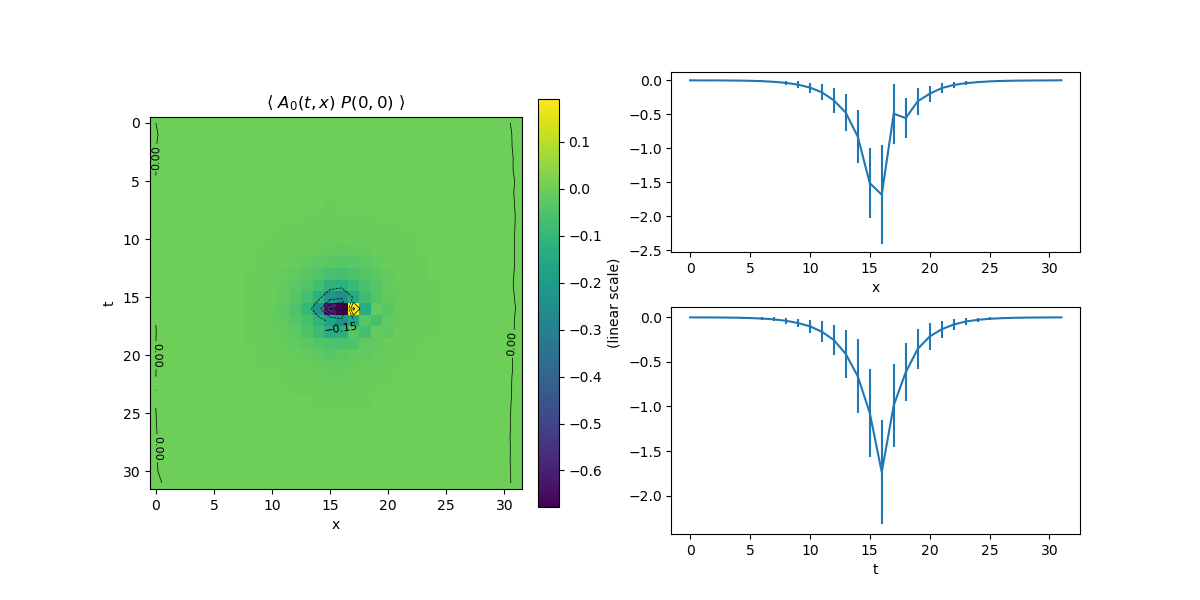
\includegraphics[width=\textwidth]{../plots/A0P.png}
    \caption{}
    \label{}
\end{figure}

\begin{figure}[H]
    \centering
    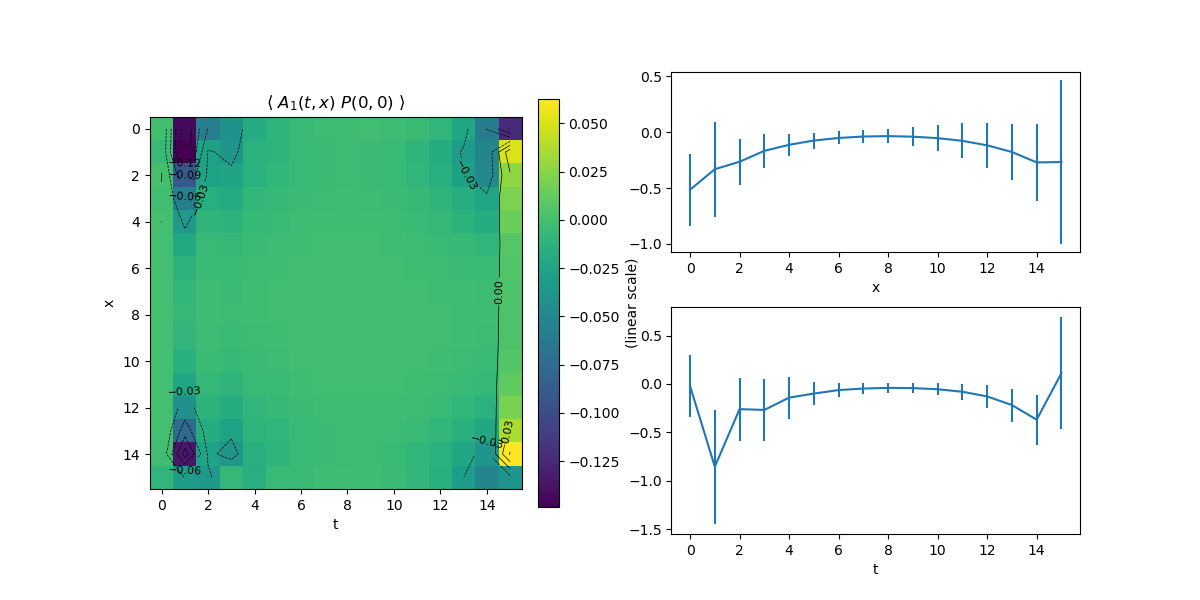
\includegraphics[width=\textwidth]{../plots/A1P.png}
    \caption{}
    \label{}
\end{figure}

\subsection{P-A correlators}

\begin{align*}
    \langle j_P^{12} (r) j_A^{\mu, 21}(0) \rangle &= \langle \bar\psi_1(r) \gamma^5 \psi_2(r) \bar\psi_2(0) \gamma^\mu \gamma^5 \psi_1(0) \rangle 
    \simeq \Tr{S(r, 0)  \gamma^5 S(0, r) \gamma^\mu \gamma^5} \\
    &= \Tr{S(r, 0)  \gamma^5 \gamma^5 S(r, 0)^\dagger \gamma^5 \gamma^\mu \gamma^5} \\
    &= -\Tr{S(r, 0) S(r, 0)^\dagger \gamma^\mu}
\end{align*}

For $\mu = 0$ we have
\begin{align*}
    \langle j_P^{12} (r) j_A^{0, 21}(0) \rangle
    &= - \Tr{ \begin{pmatrix} S_{00} & S_{01} \\ S_{10} & S_{11} \end{pmatrix} \begin{pmatrix} S_{00}^* & S_{10}^* \\ S_{01}^* & S_{11}^* \end{pmatrix} \begin{pmatrix} 0 & 1 \\ 1 & 0 \end{pmatrix} } \\
    &= - \Tr{ \begin{pmatrix} S_{00} & S_{01} \\ S_{10} & S_{11} \end{pmatrix} \begin{pmatrix} S_{10}^* & S_{00}^* \\ S_{11}^* & S_{01}^* \end{pmatrix}} \\
    &= - \Tr{\begin{pmatrix} S_{00} S_{10}^* + S_{01} S_{11}^* &  \\ & S_{10} S_{00}^* + S_{11} S_{01}^* \end{pmatrix}} \\
    &= -2 \ \Re{S_{00} S_{10}^* + S_{01} S_{11}^*}
\end{align*}

For $\mu = 1$ we have
\begin{align*}
    \langle j_P^{12} (r) j_A^{1, 21}(0) \rangle
    &= -i \ \Tr{ \begin{pmatrix} S_{00} & S_{01} \\ S_{10} & S_{11} \end{pmatrix}  \begin{pmatrix} S_{00}^* & S_{10}^* \\ S_{01}^* & S_{11}^* \end{pmatrix} \begin{pmatrix} 0 & -1 \\ 1 & 0 \end{pmatrix} } \\
    &= -i \ \Tr{ \begin{pmatrix} S_{00} & S_{01} \\ S_{10} & S_{11} \end{pmatrix} \begin{pmatrix} S_{10}^* & -S_{00}^* \\ S_{11}^* & -S_{01}^* \end{pmatrix}} \\
    &= -i \ \Tr{\begin{pmatrix} S_{00} S_{10}^* + S_{01} S_{11}^* &  \\ & -S_{10} S_{00}^* - S_{11} S_{01}^* \end{pmatrix}} \\
    &= 2 \ \Im{S_{00} S_{10}^* + S_{01} S_{11}^*}
\end{align*}

\begin{figure}[H]
    \centering
    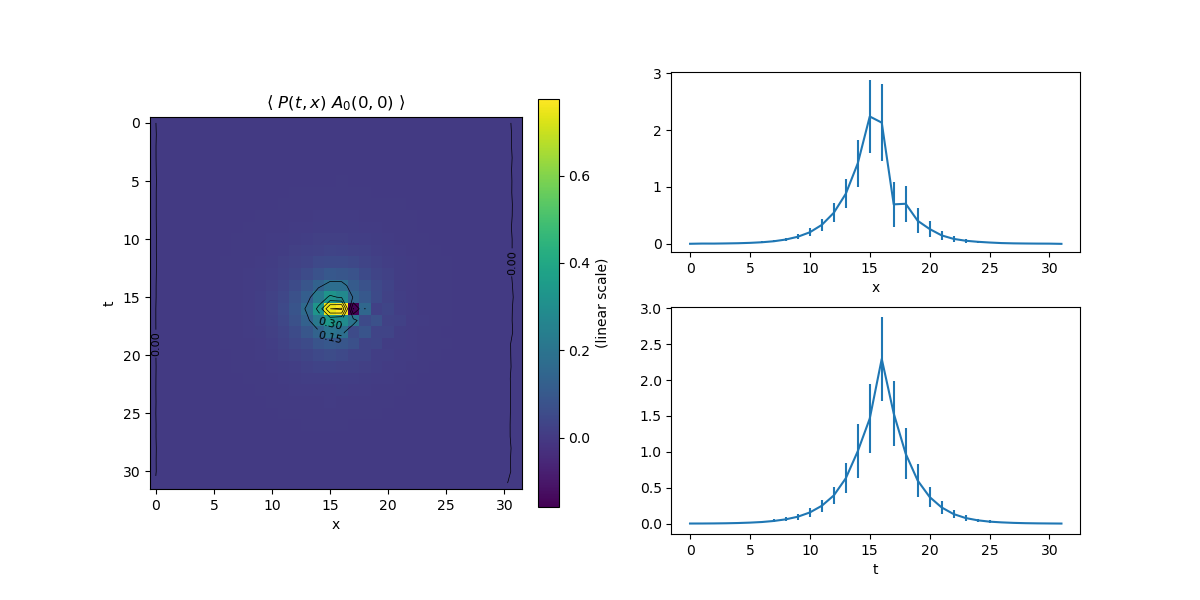
\includegraphics[width=\textwidth]{../plots/PA0.png}
    \caption{}
    \label{}
\end{figure}

\begin{figure}[H]
    \centering
    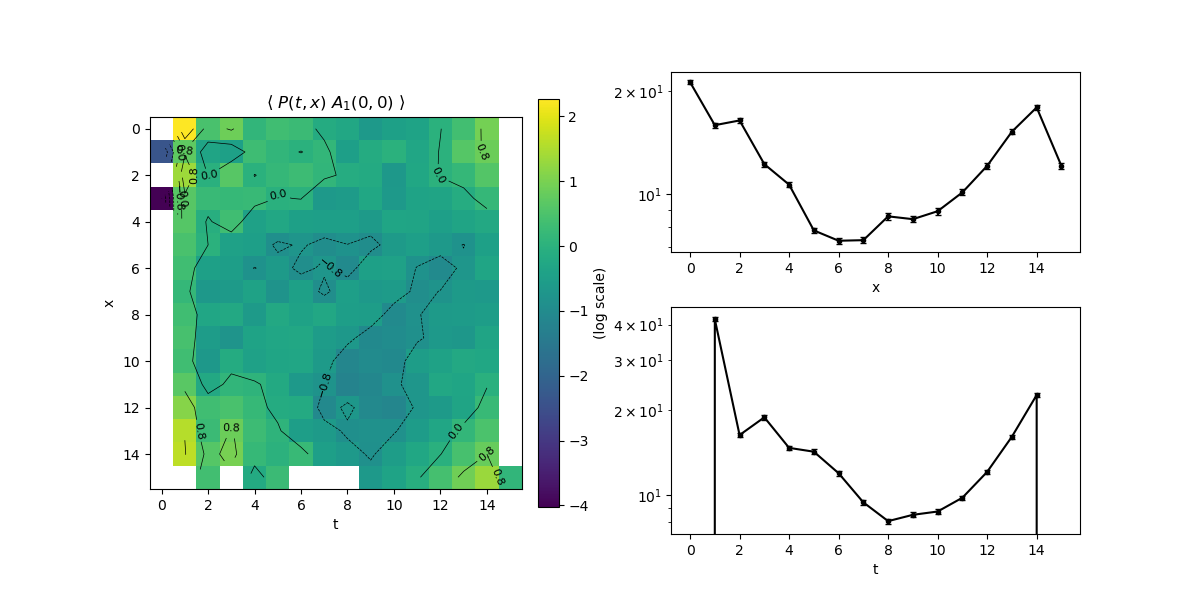
\includegraphics[width=\textwidth]{../plots/PA1.png}
    \caption{}
    \label{}
\end{figure}

\subsection{V-V correlators}

\begin{figure}[H]
    \centering
    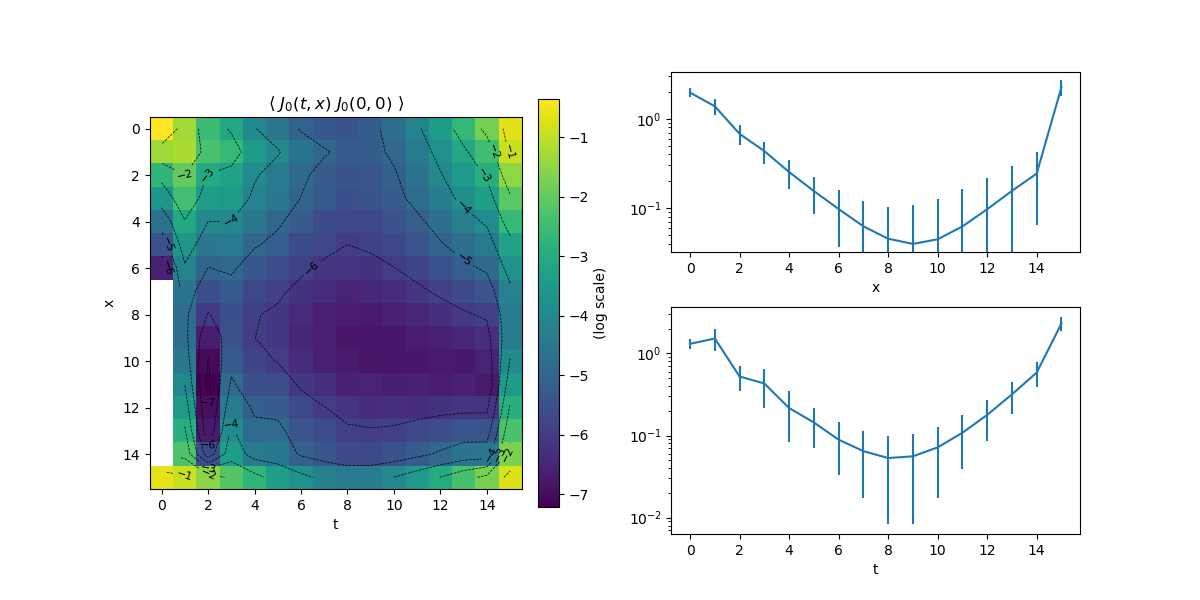
\includegraphics[width=\textwidth]{../plots/V0V0.png}
    \caption{}
    \label{}
\end{figure}

\begin{figure}[H]
    \centering
    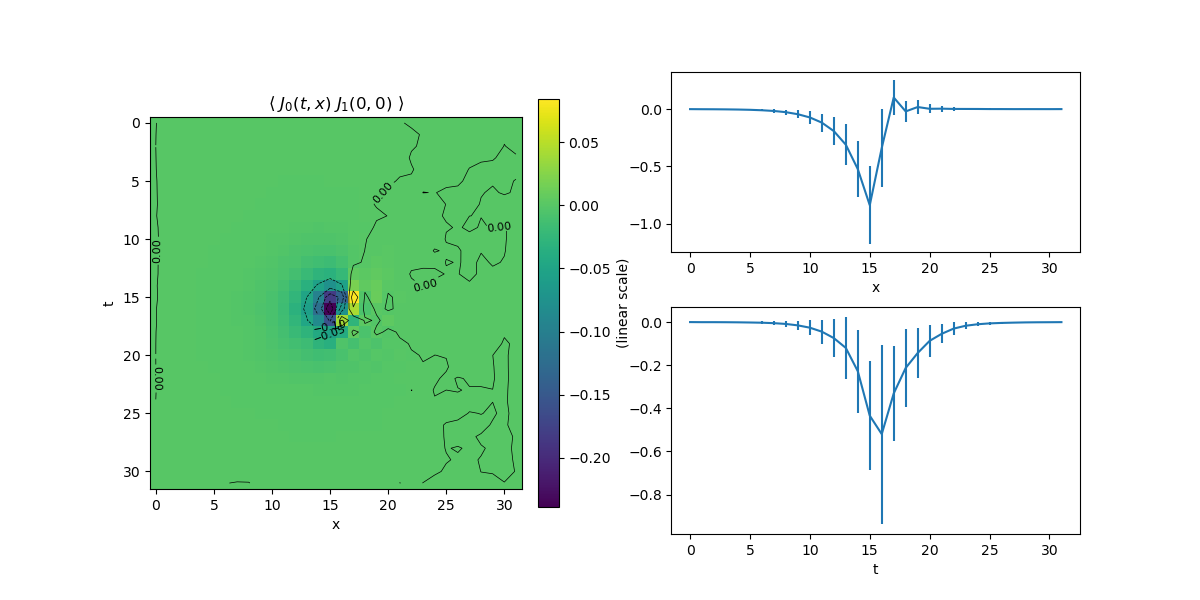
\includegraphics[width=\textwidth]{../plots/V0V1.png}
    \caption{}
    \label{}
\end{figure}

\begin{figure}[H]
    \centering
    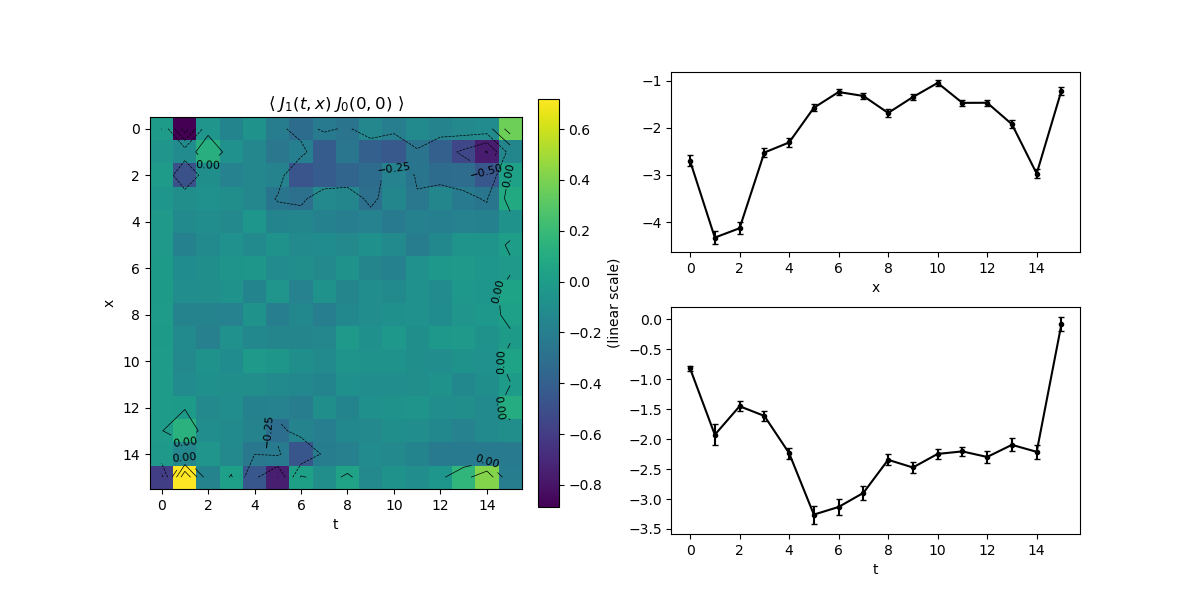
\includegraphics[width=\textwidth]{../plots/V1V0.png}
    \caption{}
    \label{}
\end{figure}

\begin{figure}[H]
    \centering
    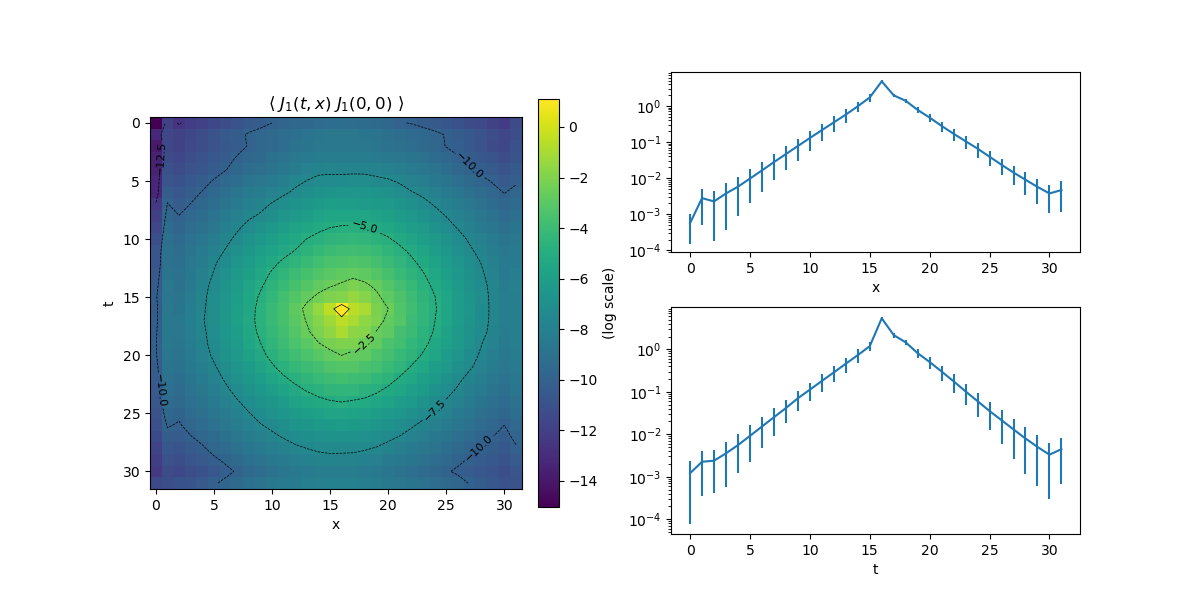
\includegraphics[width=\textwidth]{../plots/V1V1.png}
    \caption{}
    \label{}
\end{figure}

\end{document}